% --- PAGE 37: HALF-TITLE SYSTEM DESIGN ---
\vspace*{\fill}
\begin{center}
  {\fontsize{18pt}{24pt}\selectfont\bfseries SYSTEM DESIGN\par}
\end{center}
\vspace*{\fill}
\newpage

% --- PAGE 38: CHAPTER 6 SYSTEM DESIGN ---
\begin{center}
  {\fontsize{16pt}{20pt}\selectfont\bfseries CHAPTER 6\par}
  \vspace{0.3cm}
  {\fontsize{16pt}{20pt}\selectfont\bfseries SYSTEM DESIGN\par}
\end{center}
\vspace{0.4cm}

{\fontsize{14pt}{18pt}\selectfont\bfseries 6.1 INTRODUCTION\par}
\vspace{0.2cm}

{\fontsize{12pt}{18pt}\selectfont
The System Design phase translates the functional and architectural specifications of the \textbf{VSBEC IT Vault} platform into formal visual design models. These structural and behavioral models define how components, data entities, and system actors interact across the continuous academic lifecycle.

This chapter constructs six standard UML and process models: Class Diagrams defining the relational domain entities; Use Case Diagrams modeling actor permissions; Sequence Diagrams illustrating chronological message exchanges during task submission and compilation; Activity Diagrams mapping decision workflows; and Level 0/1 Data Flow Diagrams (DFD) formalizing information transformation across database and cloud storage boundaries.

\vspace{0.3cm}
{\fontsize{14pt}{18pt}\selectfont\bfseries 6.2 CLASS DIAGRAM\par}
\vspace{0.2cm}
The Class Diagram models the static structure of the platform's domain entities. In this system, core entity models include \texttt{User}, \texttt{Department}, \texttt{ClassGroup}, \texttt{Task}, \texttt{TaskSubmission}, \texttt{SubmissionReview}, \texttt{Team}, \texttt{LeetCodeTarget}, \texttt{GitHubDailyCommit}, \texttt{CodingAssessment}, and \texttt{NotificationPreference}.

\vspace{0.2cm}
\noindent\textbf{OBJECTIVES:}
\begin{enumerate}[noitemsep,topsep=2pt,leftmargin=*]
  \item Model entity attributes, primary keys, and methods corresponding to the 13 PostgreSQL schema tables.
  \item Establish structural associations, composition rules, and foreign key constraints across entities.
\end{enumerate}\par}
\newpage

% --- PAGE 39: CLASS DIAGRAM ---
\begin{enumerate}[noitemsep,topsep=2pt,leftmargin=*]
  \setcounter{enumi}{2}
  \item Represent multi-tier review relationships linking student submissions to coordinator, advisor, and HOD reviews.
  \item Model coding assessment entities including question banks, test cases, and candidate submission records.
  \item Map telemetry entities storing daily LeetCode solve counts and GitHub commit records.
  \item Formalize role-based polymorphism across Supreme Admin, HOD, Faculty, Student, and Industry entities.
  \item Ensure modular separation between local persistent entities and external Cloudinary/Judge0 assets.
\end{enumerate}

\vspace{0.2cm}
\begin{figure}[H]
  \centering
  \setlength{\fboxrule}{0.8pt}%
  \fcolorbox{black!20}{white}{%
    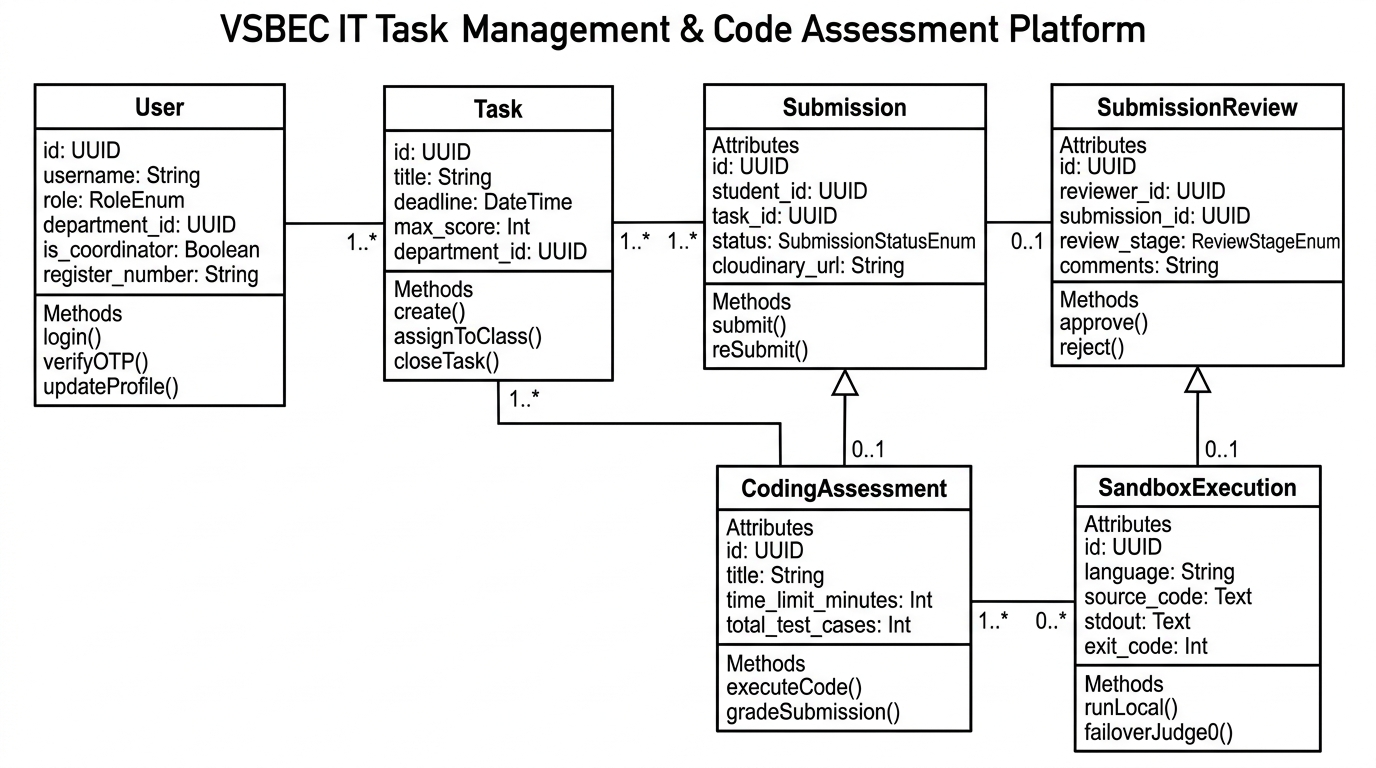
\includegraphics[width=0.92\textwidth,height=8.8cm,keepaspectratio]{images/class_diagram.png}%
  }\par
  \vspace{6pt}
  {\centering\fontsize{12pt}{16pt}\selectfont\bfseries Fig 6.1 Class Diagram\par}
\end{figure}
\newpage

% --- PAGE 40: SECTION 6.3 USE CASE DIAGRAM ---
{\fontsize{14pt}{18pt}\selectfont\bfseries 6.3 USE CASE DIAGRAM\par}
\vspace{0.3cm}

{\fontsize{12pt}{18pt}\selectfont
A Use Case Diagram captures system functional requirements from the perspective of external actors. In the VSBEC IT Vault platform, primary human actors include \textbf{Students}, \textbf{Student Coordinators}, \textbf{Faculty Class Advisors}, the \textbf{Head of the Department (HOD)}, \textbf{Supreme Administrators}, and \textbf{Industry Partners}, alongside automated system actors (Cron Telemetry Daemons and Telegram Bots).

\vspace{0.3cm}
{\fontsize{14pt}{18pt}\selectfont\bfseries OBJECTIVES:\par}
\vspace{0.2cm}
\begin{enumerate}[noitemsep,topsep=2pt,leftmargin=*]
  \item Define student use cases: Task submission, Monaco code compilation, LeetCode profile linking, and team tasks.
  \item Specify coordinator use cases: Peer-level rubric review, submission verification, and class progress auditing.
  \item Map faculty advisor use cases: Task creation, secondary verification, deadline extension, and Telegram dispatch.
  \item Delineate HOD use cases: Department-wide task sign-off, section analytics, and faculty performance auditing.
  \item Define industry partner use cases: Assessment creation, custom test case authoring, and candidate shortlisting.
  \item Model automated daemon use cases: Nightly GraphQL telemetry polling and scheduled notification broadcasts.
\end{enumerate}\par}
\newpage

% --- PAGE 41: FIG 6.2 USE CASE DIAGRAM ---
\begin{figure}[H]
  \centering
  \setlength{\fboxrule}{0.8pt}%
  \fcolorbox{black!20}{white}{%
    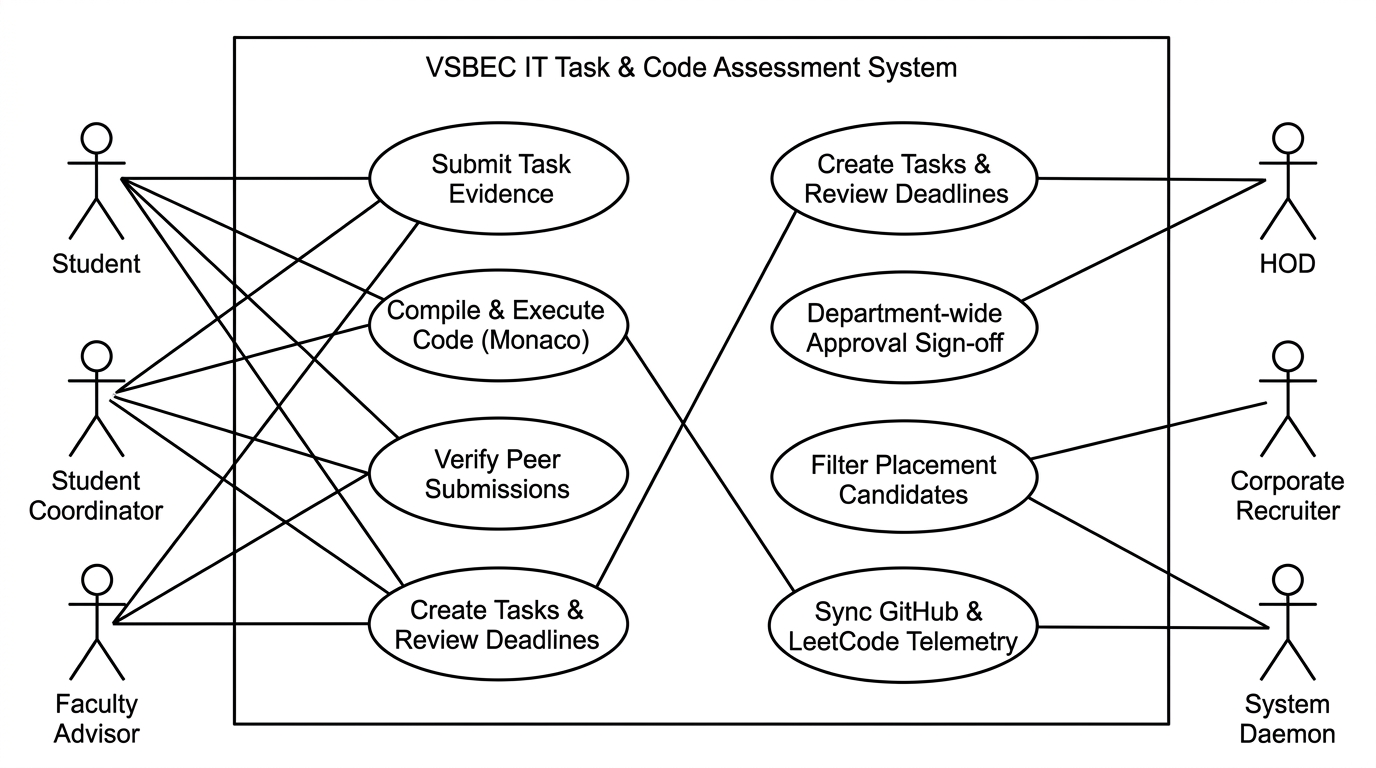
\includegraphics[width=0.92\textwidth,height=8.8cm,keepaspectratio]{images/use_case_diagram.png}%
  }\par
  \vspace{6pt}
  {\centering\fontsize{12pt}{16pt}\selectfont\bfseries Fig 6.2 Use Case Diagram\par}
\end{figure}

\vspace{0.3cm}
{\fontsize{14pt}{18pt}\selectfont\bfseries 6.4 SEQUENCE DIAGRAM\par}
\vspace{0.2cm}
{\fontsize{12pt}{18pt}\selectfont
A Sequence Diagram models the chronological exchange of messages between client components, API controllers, database services, and external microservices during a specific business transaction.\par}
\newpage

% --- PAGE 42: FIG 6.3 SEQUENCE DIAGRAM ---
{\fontsize{12pt}{18pt}\selectfont
In this system, the primary sequence diagram illustrates the complete end-to-end lifecycle of a proctored coding assessment: the student launches the Monaco IDE test, the proctoring engine initializes webcam PIP streams, source code is submitted to the backend API, the sandbox spawns isolated execution child processes, test case outputs are validated against hidden assertions, and final scorecards are persisted in PostgreSQL. The sequence diagram captures message timings, error recovery, and cloud failover branches.\par}

\vspace{0.2cm}
\begin{figure}[H]
  \centering
  \setlength{\fboxrule}{0.8pt}%
  \fcolorbox{black!20}{white}{%
    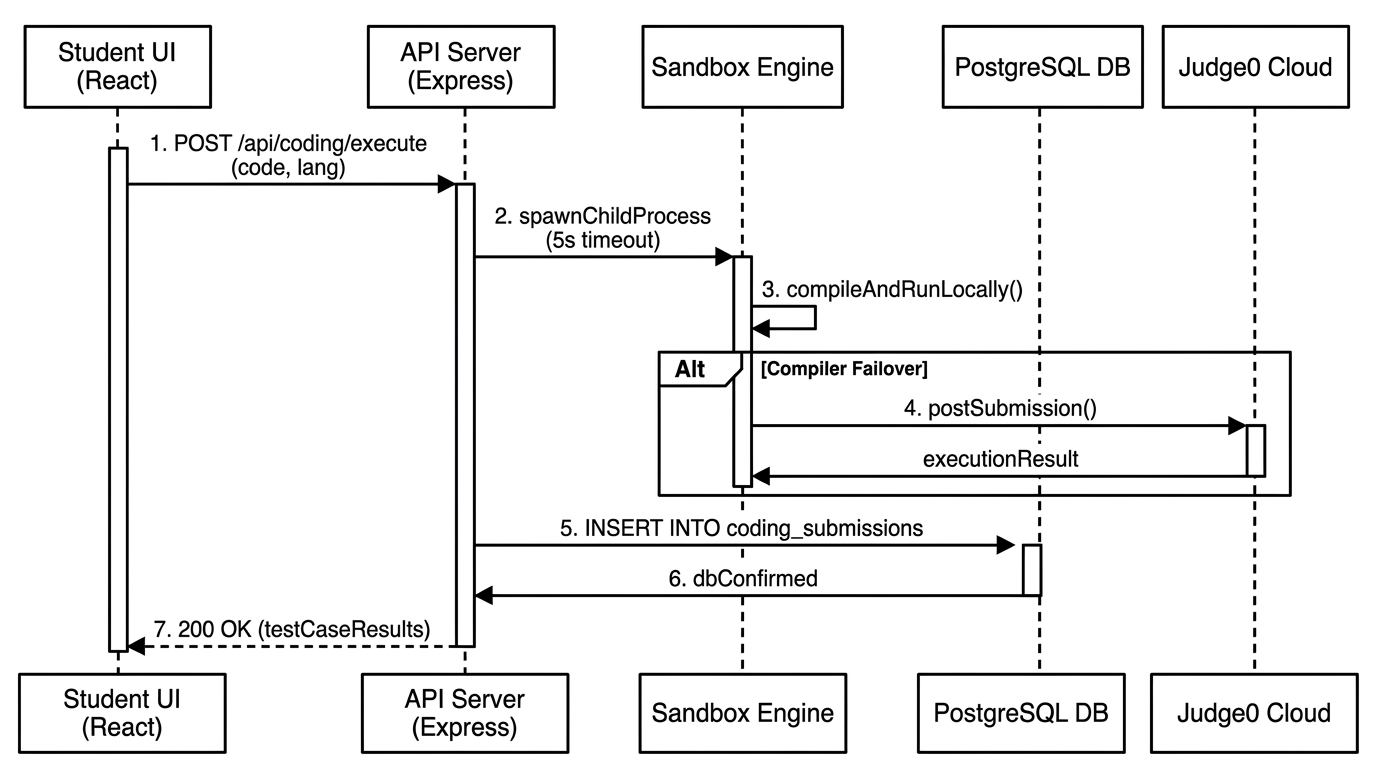
\includegraphics[width=0.92\textwidth,height=8.8cm,keepaspectratio]{images/sequence_diagram.png}%
  }\par
  \vspace{6pt}
  {\centering\fontsize{12pt}{16pt}\selectfont\bfseries Fig 6.3 Sequence Diagram\par}
\end{figure}
\newpage

% --- PAGE 43: SECTION 6.5 ACTIVITY DIAGRAM ---
{\fontsize{14pt}{18pt}\selectfont\bfseries 6.5 ACTIVITY DIAGRAM\par}
\vspace{0.2cm}

{\fontsize{12pt}{18pt}\selectfont
The Activity Diagram models the step-by-step control flow and decision logic of the 3-tier academic task verification pipeline. It visually represents branch conditions (e.g., submission accepted vs. rejected with feedback), coordinator peer audits, faculty reviews, resubmission loops, and automated notification triggers.\par}

\vspace{0.2cm}
\begin{figure}[H]
  \centering
  \setlength{\fboxrule}{0.8pt}%
  \fcolorbox{black!20}{white}{%
    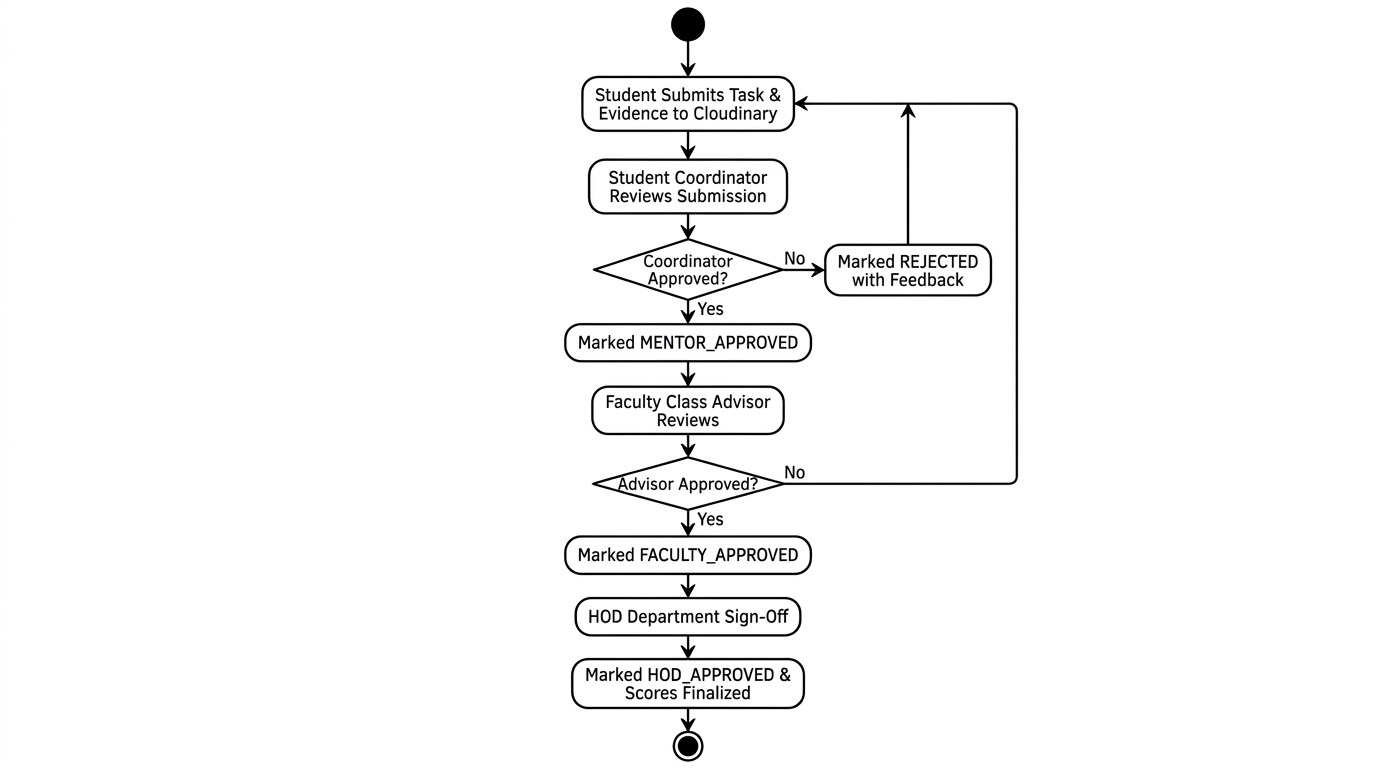
\includegraphics[width=0.92\textwidth,height=8.8cm,keepaspectratio]{images/activity_diagram.png}%
  }\par
  \vspace{6pt}
  {\centering\fontsize{12pt}{16pt}\selectfont\bfseries Fig 6.4 Activity Diagram\par}
\end{figure}
\newpage

% --- PAGE 44: SECTION 6.6 DATA FLOW DIAGRAM ---
{\fontsize{14pt}{18pt}\selectfont\bfseries 6.6 DATA FLOW DIAGRAM (DFD LEVEL 0 \& LEVEL 1)\par}
\vspace{0.2cm}

{\fontsize{12pt}{18pt}\selectfont
A Data Flow Diagram (DFD) formalizes information transformation across logical processing boundaries. Level 0 (Context Diagram) depicts the platform as a central process interacting with external entities (Students, Faculty, Industry, Telegram, LeetCode, GitHub). Level 1 decomposes the system into six core functional processes: Authentication, Task Ingestion, Sandboxed Evaluation, Telemetry Harvesting, Alert Relay, and Placement Export.\par}

\vspace{0.2cm}
\begin{figure}[H]
  \centering
  \setlength{\fboxrule}{0.8pt}%
  \fcolorbox{black!20}{white}{%
    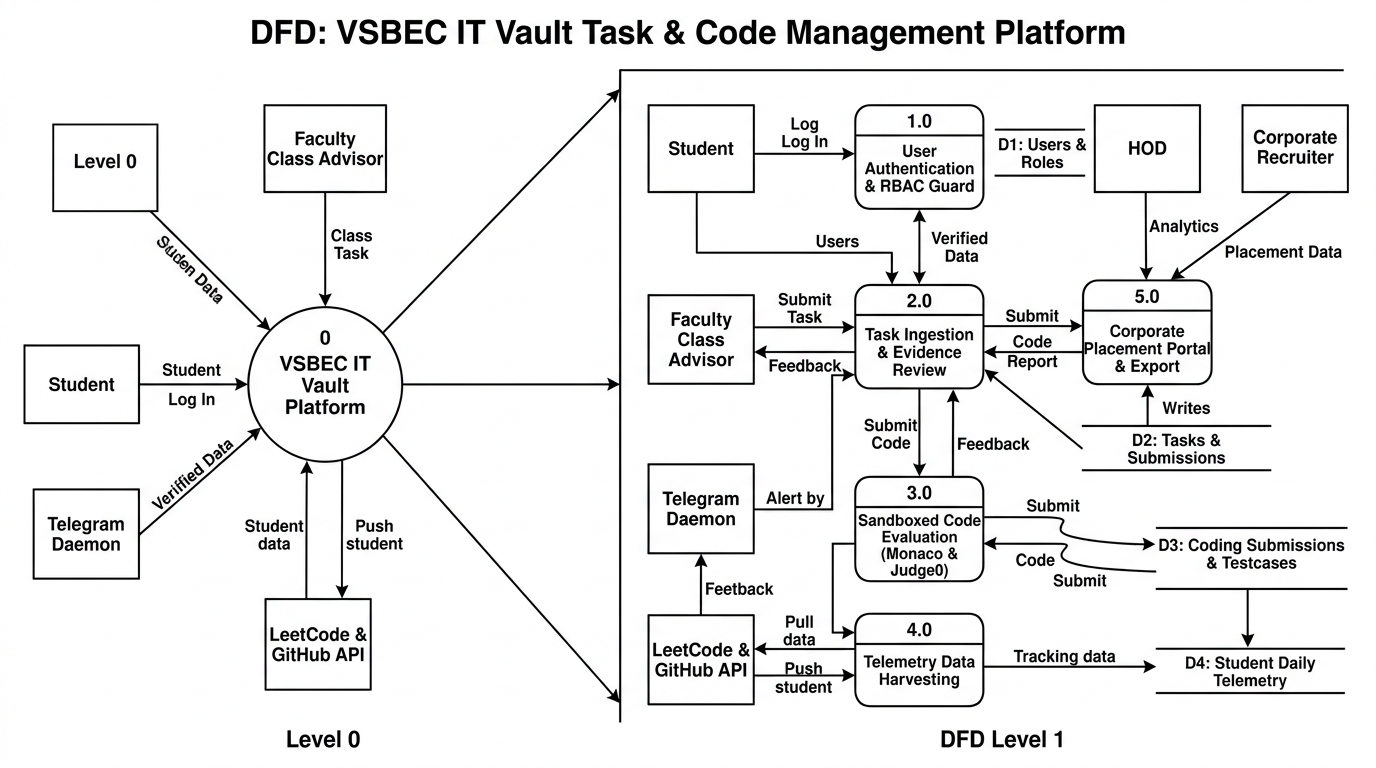
\includegraphics[width=0.92\textwidth,height=8.8cm,keepaspectratio]{images/dfd_diagram.png}%
  }\par
  \vspace{6pt}
  {\centering\fontsize{12pt}{16pt}\selectfont\bfseries Fig 6.5 Data Flow Diagram\par}
\end{figure}
\newpage
